\section{条件分布的积分}
\label{sec:cdis-integration}

固定观测值$y$，$K(y,\cdot)$是一个普通的概率测度，可以对它积分。这样得到的$\int g(x)\,K(y,\mathrm{d}x)$是“观测为$y$时$g(X)$的平均”。它与第~\ref{chap:conditional-expectation}章的条件期望$\mathbb{E}[g(X)\mid Y]$是什么关系？这一节证明，在可积条件下两者几乎必然相等，再用这个表示计算条件矩。

条件期望仍以第~\ref{chap:conditional-expectation}章的积分刻画为定义，它对任何可积随机变量都存在；下面的表示只在正则条件分布存在时才可用，它提供的是一个计算方法和一个对每个$y$都有定义的版本。

\subsection{条件期望的积分表示}
\label{sec:cdis-integral-representation}

\begin{theorem}[条件期望的积分表示]
\label{thm:cdis-integral-representation}
设$K$是给定$Y$时$X$的正则条件分布，$g:\mathcal{X}\to\mathbb{R}$可测，$\mathbb{E}\lvert g(X)\rvert<\infty$。则对$P_Y$几乎每个$y$，$\int\lvert g(x)\rvert\,K(y,\mathrm{d}x)<\infty$，并且
\begin{equation}
 \mathbb{E}[g(X)\mid Y]=\int g(x)\,K(Y,\mathrm{d}x)\quad\text{几乎必然}.
 \label{eq:cdis-integral-representation}
\end{equation}
在使积分不收敛的$P_Y$零测集上，右边可以取任意常数，例如$0$。
\end{theorem}

证明沿着积分本身的构造进行：先对指示函数，再对简单函数，然后用单调极限处理非负函数，最后拆成正负两部分。两边的每一步分别用测度积分的性质与条件期望的性质。

\begin{proof}
记$(Kg)(y)=\int g(x)\,K(y,\mathrm{d}x)$。

第一步，$g=\mathbf{1}_{A}$。此时$(Kg)(Y)=K(Y,A)$，式~\eqref{eq:cdis-integral-representation}就是正则条件分布的定义~\eqref{eq:cdis-regular}。

第二步，$g=\sum_{i=1}^{m}c_i\mathbf{1}_{A_i}$是简单函数。左边由条件期望的线性，右边由积分的线性，都拆成各项之和，各项由第一步相等。

第三步，$g\geq0$。取简单函数$g_n=\min\{n,\ 2^{-n}\lfloor2^{n}g\rfloor\}$，它们非负、递增地收敛到$g$。对每个固定的$y$，由单调收敛定理（对测度$K(y,\cdot)$），
\[
 (Kg_n)(y)\uparrow(Kg)(y)\in[0,\infty],
\]
所以$Kg$作为可测函数的极限是可测的。另一方面$g(X)$可积，由引理~\ref{lem:cdis-conditional-monotone}，$\mathbb{E}[g_n(X)\mid Y]\uparrow\mathbb{E}[g(X)\mid Y]$几乎必然。由第二步两列的每一项几乎必然相等，极限也几乎必然相等，这就是式~\eqref{eq:cdis-integral-representation}。

再看有限性。对$(Kg_n)(Y)$取期望，用全期望公式与第二步，$\mathbb{E}[(Kg_n)(Y)]=\mathbb{E}[g_n(X)]$；两边对$n$用单调收敛定理，得到
\[
 \int(Kg)(y)\,P_Y(\mathrm{d}y)=\mathbb{E}[g(X)]<\infty .
\]
非负函数的积分有限，它就只能在一个$P_Y$零测集上取$+\infty$。

第四步，一般的可积$g$。写$g=g^{+}-g^{-}$，两部分都非负且$g^{\pm}(X)$可积。由第三步，$Kg^{+}$与$Kg^{-}$在一个共同的$P_Y$零测集之外都有限，在这个零测集之外，$\lvert g\rvert$关于$K(y,\cdot)$的积分是$(Kg^{+})(y)+(Kg^{-})(y)<\infty$，并且$(Kg)(y)=(Kg^{+})(y)-(Kg^{-})(y)$。再由条件期望的线性，
\[
 \mathbb{E}[g(X)\mid Y]=\mathbb{E}[g^{+}(X)\mid Y]-\mathbb{E}[g^{-}(X)\mid Y]=(Kg)(Y)\quad\text{几乎必然}. \qedhere
\]
\end{proof}

第三步的单调逼近可以具体地看。三角形模型中取$y=0.4$，$K(0.4,\cdot)$是$[0.4,1]$上的均匀分布，取$g(x)=x^{2}$。精确值是
\[
 \int x^{2}\,K(0.4,\mathrm{d}x)=\frac{1}{0.6}\int_{0.4}^{1}x^{2}\,\mathrm{d}x=\frac{1-0.064}{1.8}=0.52 .
\]
$g$不超过$1$，所以$g_n=2^{-n}\lfloor2^{n}g\rfloor$，它是$2^{n}$级的阶梯。$n=1,2,3,4$时，阶梯函数在$K(0.4,\cdot)$下的积分依次约为
\[
 0.244,\qquad 0.386,\qquad 0.456,\qquad 0.488,
\]
递增地逼近$0.52$，见图~\ref{fig:cdis-simple-approx}。

\begin{BookInlineFigure}
  \centering
  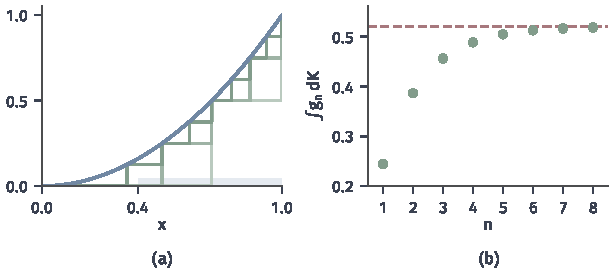
\includegraphics[width=104mm]{figures/07-probability/02-measure-theoretic-probability/matplotlib/cdis-simple-approx/figure.pdf}
  \caption{用简单函数逼近条件分布下的积分，三角形模型，$y=0.4$。(a)蓝线是$g(x)=x^{2}$，绿色阶梯是$g_n=2^{-n}\lfloor2^{n}g\rfloor$（$n=1,2,3$，颜色由浅到深），浅蓝区间$[0.4,1]$是$K(0.4,\cdot)$的支撑。(b)绿点是$\int g_n\,\mathrm{d}K(0.4,\cdot)$，$n=1,\dots,8$，红色虚线是极限$0.52$。}
  \label{fig:cdis-simple-approx}
\end{BookInlineFigure}

\paragraph{离散与密度的情形}
把定理~\ref{thm:cdis-integral-representation}用于前面的两类模型，就得到熟悉的公式。有概率表时，对$p_Y(y)>0$，
\[
 \mathbb{E}[g(X)\mid Y=y]=\sum_{x}g(x)\,\frac{p_{X,Y}(x,y)}{p_Y(y)} ;
\]
有联合密度时，由定理~\ref{thm:cdis-density-version}，对$0<f_Y(y)<\infty$，
\[
 \mathbb{E}[g(X)\mid Y=y]=\int g(x)\,\frac{f_{X,Y}(x,y)}{f_Y(y)}\,\mathrm{d}x .
\]
第~\ref{chap:random-vectors}章按这两个公式计算条件均值，当时它们只是“组内平均”的计算规则；现在可以说，它们给出的函数代入$Y$后正是条件期望的一个版本，第~\ref{chap:conditional-expectation}章关于条件期望的全部性质都可以用于它们。

三角形模型中，对$0\leq y<1$，
\[
 \mathbb{E}[g(X)\mid Y=y]=\frac{1}{1-y}\int_{y}^{1}g(x)\,\mathrm{d}x ,
\]
即$[y,1]$上$g$的平均值。取$g(x)=x$得到$(1+y)/2$，与第~\ref{chap:random-vectors}章的结果一致。

\subsection{条件矩的计算}
\label{sec:cdis-conditional-moments}

设$X$是实随机变量。取$g(x)=x^{k}$或$g(x)=\lvert x\rvert^{p}$，在相应的矩存在时，定理~\ref{thm:cdis-integral-representation}给出条件矩的积分公式：若$\mathbb{E}\lvert X\rvert^{p}<\infty$，$p>0$，则
\begin{equation}
 \mathbb{E}\bigl[\lvert X\rvert^{p}\bigm|Y\bigr]=\int\lvert x\rvert^{p}\,K(Y,\mathrm{d}x)<\infty\quad\text{几乎必然},
 \label{eq:cdis-conditional-abs-moment}
\end{equation}
若$k\leq p$是正整数，则几乎必然
\[
 \mathbb{E}[X^{k}\mid Y]=\int x^{k}\,K(Y,\mathrm{d}x),
\]
其中$\lvert x\rvert^{k}\leq1+\lvert x\rvert^{p}$保证$X^{k}$可积。这些量称为给定$Y$的\term{条件矩}（conditional moment）。

\paragraph{条件方差}
第~\ref{chap:conditional-expectation}章对$\mathbb{E}[X^{2}]<\infty$定义了条件方差
\[
 \operatorname{Var}(X\mid Y)=\mathbb{E}\bigl[(X-\mathbb{E}[X\mid Y])^{2}\bigm|Y\bigr].
\]
记$m(y)=\int x\,K(y,\mathrm{d}x)$，它在$P_Y$几乎每个$y$处有限，并且$m(Y)=\mathbb{E}[X\mid Y]$几乎必然。条件方差可以写成条件分布的方差。

\begin{theorem}[条件方差的积分表示]
\label{thm:cdis-conditional-variance}
设$\mathbb{E}[X^{2}]<\infty$，$K$是给定$Y$时$X$的正则条件分布。则几乎必然
\begin{equation}
 \operatorname{Var}(X\mid Y)=\int\bigl(x-m(Y)\bigr)^{2}\,K(Y,\mathrm{d}x)=\int x^{2}\,K(Y,\mathrm{d}x)-m(Y)^{2}.
 \label{eq:cdis-conditional-variance}
\end{equation}
\end{theorem}

\begin{proof}
由式~\eqref{eq:cdis-conditional-abs-moment}，存在$P_Y$零测集$N$，使$y\notin N$时$\int x^{2}\,K(y,\mathrm{d}x)<\infty$，从而$m(y)$有限。对这样的$y$，$K(y,\cdot)$是二阶矩有限的分布，展开平方得到
\[
 \begin{aligned}
 \int\bigl(x-m(y)\bigr)^{2}K(y,\mathrm{d}x)&=\int x^{2}K(y,\mathrm{d}x)-2m(y)^{2}+m(y)^{2}\\
 &=\int x^{2}K(y,\mathrm{d}x)-m(y)^{2}.
 \end{aligned}
\]
这是式~\eqref{eq:cdis-conditional-variance}的第二个等号。

另一方面，展开条件方差的定义。$m(Y)$与$X$都平方可积，由Cauchy--Schwarz不等式$m(Y)X$可积，于是可以用线性和提取已知量：
\[
 \begin{aligned}
 \operatorname{Var}(X\mid Y)&=\mathbb{E}[X^{2}\mid Y]-2m(Y)\,\mathbb{E}[X\mid Y]+m(Y)^{2}\\
 &=\mathbb{E}[X^{2}\mid Y]-m(Y)^{2}.
 \end{aligned}
\]
由式~\eqref{eq:cdis-conditional-abs-moment}取$p=2$，右边第一项$\mathbb{E}[X^{2}\mid Y]$几乎必然等于$\int x^{2}K(Y,\mathrm{d}x)$，两式相同。
\end{proof}

式~\eqref{eq:cdis-conditional-variance}就是“方差等于二阶矩减均值平方”对每个条件分布分别使用。它把条件方差从一个由积分刻画定义的随机变量，变成了每个观测值处一个具体分布的方差。

\paragraph{正面概率随机的硬币}
设$U\sim\operatorname{Unif}(0,1)$，给定$U=u$时把一枚正面概率为$u$的硬币独立地抛$n$次，$N$是正面次数。这句话本身就是用概率核描述的模型：
\[
 K(u,\{k\})=\binom{n}{k}u^{k}(1-u)^{n-k},\qquad k=0,1,\dots,n ,
\]
即给定$U=u$时$N\sim\operatorname{Bin}(n,u)$。联合规律由$U$的分布和这个核共同确定，第~\ref{sec:cdis-joint}节说明为什么这样确定的联合规律唯一，并且这个核就是它的正则条件分布。

二项分布的均值与方差在第~\ref{chap:common-distributions}章已经算出，代入式~\eqref{eq:cdis-integral-representation}与式~\eqref{eq:cdis-conditional-variance}，
\[
 \mathbb{E}[N\mid U]=nU,\qquad \operatorname{Var}(N\mid U)=nU(1-U).
\]
条件均值随$U$线性增长，条件方差在$U=\tfrac12$处最大，在两端趋于零。

由全方差公式，总方差是条件方差的平均加上条件均值的方差。用$\mathbb{E}[U]=\tfrac12$、$\mathbb{E}[U^{2}]=\tfrac13$、$\operatorname{Var}(U)=\tfrac1{12}$，
\[
 \mathbb{E}\bigl[nU(1-U)\bigr]=n\Bigl(\frac12-\frac13\Bigr)=\frac n6,\qquad \operatorname{Var}(nU)=\frac{n^{2}}{12}.
\]
于是
\[
 \operatorname{Var}(N)=\frac n6+\frac{n^{2}}{12}=\frac{n(n+2)}{12}.
\]
$n=10$时组内部分为$\tfrac53\approx1.67$，组间部分为$\tfrac{25}{3}\approx8.33$，总方差为$10$。组间部分随$n^{2}$增长，占了大头：抛得越多，正面次数的波动主要来自硬币本身的不确定，而不是给定硬币后的随机性。图~\ref{fig:cdis-coin-moments}画出这两部分。第~\ref{sec:cdis-mixture}小节将看到$N$在$\{0,1,\dots,n\}$上均匀分布，其方差$\bigl((n+1)^{2}-1\bigr)/12$与这里的结果相同。

\begin{BookInlineFigure}
  \centering
  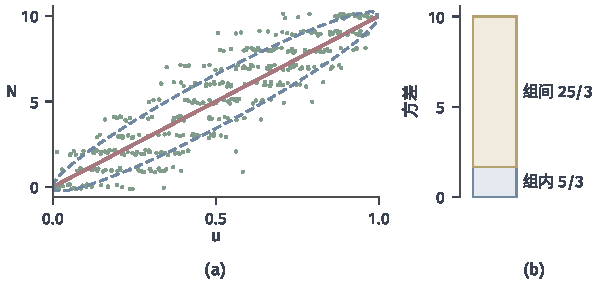
\includegraphics[width=104mm]{figures/07-probability/02-measure-theoretic-probability/matplotlib/cdis-coin-moments/figure.pdf}
  \caption{正面概率随机的硬币，$n=10$。(a)绿点是固定种子$3$模拟的$400$对$(U,N)$，纵向略加抖动以便看清；红线是条件均值$10u$，蓝色虚线是条件均值加减一个条件标准差$\sqrt{10u(1-u)}$。(b)总方差$10$的分解：浅蓝为组内部分$\tfrac53$，浅黄为组间部分$\tfrac{25}{3}$。}
  \label{fig:cdis-coin-moments}
\end{BookInlineFigure}

\paragraph{有限性只在几乎处处的意义下成立}
式~\eqref{eq:cdis-conditional-abs-moment}说整体矩有限保证条件矩\emph{几乎处处}有限，不能加强为对每个观测值有限。三角形模型中，把$y=\tfrac12$处的分布换成标准Cauchy分布，由第~\ref{sec:cdis-uniqueness}小节，所得的核仍是正则条件分布；可是Cauchy分布的绝对一阶矩是无穷，$\lvert x\rvert$关于$K'(\tfrac12,\cdot)$的积分发散，尽管$X$有界。哪个零测点上的条件矩有限，联合规律管不着。

反方向同样不成立：每个观测值上的条件矩有限，不能推出整体矩有限。设$Y\sim\operatorname{Unif}(0,1)$，给定$Y=y$时$X\sim\operatorname{Exp}(y)$，即率参数为$y$的指数分布。对每个$y\in(0,1)$，条件均值有限，
\[
 \int x\,K(y,\mathrm{d}x)=\frac1y<\infty .
\]
可是定理~\ref{thm:cdis-integral-representation}证明第三步中关于有限性的论证只用到简单函数与单调收敛，对任何非负$g$都成立，结果允许取$+\infty$：$\int(Kg)\,\mathrm{d}P_Y=\mathbb{E}[g(X)]$。取$g(x)=x$，
\[
 \mathbb{E}[X]=\int_0^1\frac1y\,\mathrm{d}y=+\infty .
\]
条件均值$1/y$在$y\to0$附近增长得太快，加权平均发散，见图~\ref{fig:cdis-moment-directions}。此时$X$不可积，第~\ref{chap:conditional-expectation}章的条件期望没有定义，只能说核的积分$1/y$是一个逐点有限的函数。

\begin{BookInlineFigure}
  \centering
  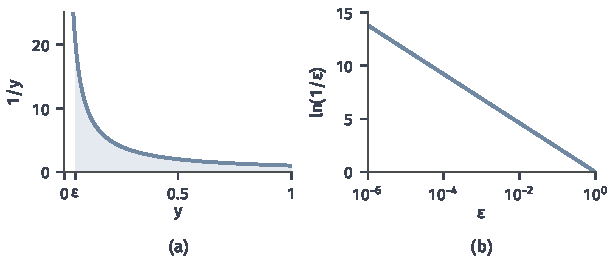
\includegraphics[width=104mm]{figures/07-probability/02-measure-theoretic-probability/matplotlib/cdis-moment-directions/figure.pdf}
  \caption{逐点有限的条件均值不保证整体可积。$Y\sim\operatorname{Unif}(0,1)$，给定$Y=y$时$X\sim\operatorname{Exp}(y)$。(a)蓝线是条件均值$1/y$，浅蓝区域是$[\varepsilon,1]$上的面积，$\varepsilon=0.05$。(b)蓝线是截断积分$\int_{\varepsilon}^{1}y^{-1}\,\mathrm{d}y=\ln(1/\varepsilon)$，横轴按对数刻度，$\varepsilon\to0$时无界增长。}
  \label{fig:cdis-moment-directions}
\end{BookInlineFigure}
